\documentclass[11pt, oneside]{article} 
\usepackage{geometry}
\geometry{letterpaper} 
\usepackage{graphicx}
	
\usepackage{amssymb}
\usepackage{amsmath}
\usepackage{parskip}
\usepackage{color}
\usepackage{hyperref}

\graphicspath{{/Users/telliott_admin/Tex/png/}}
% \begin{center} 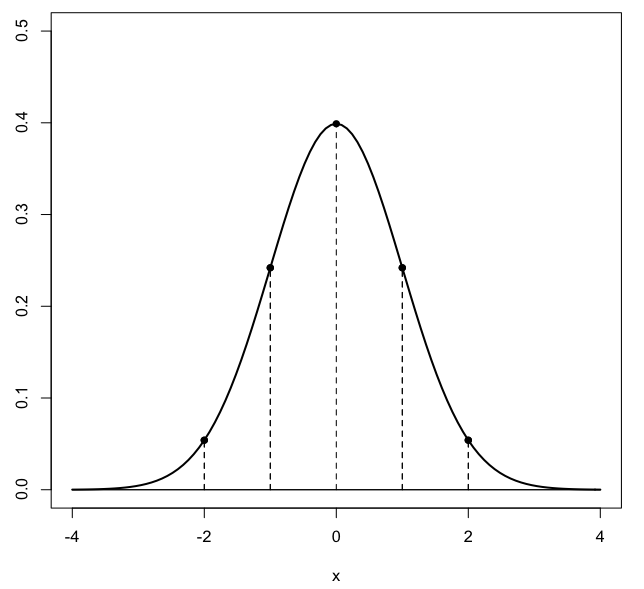
\includegraphics [scale=0.4] {gauss3.png} \end{center}

\title{Double integrals}
\date{}

\begin{document}
\maketitle
\Large

Double integrals start with a function of two variables, say $f(x,y)$.  Think of this as a surface with height $z=f(x,y)$, it could be a sloping roof or something more irregular, but still smooth.

\begin{center} 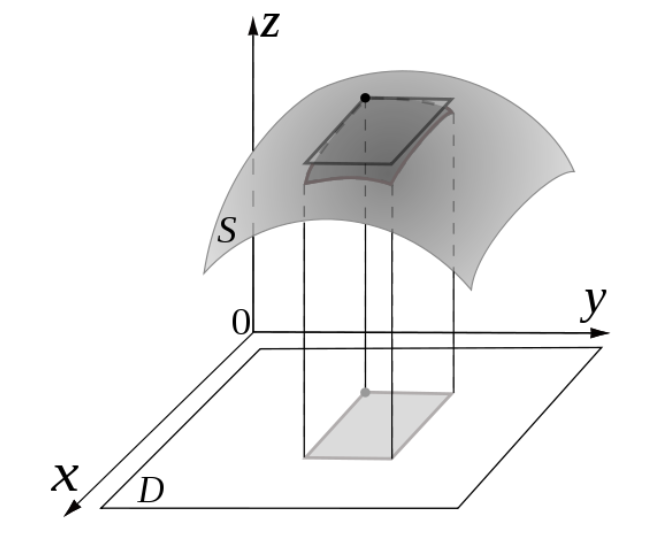
\includegraphics [scale=0.3] {double_int.png} \end{center}

Integration is performed over a region in the xy-plane that is the \emph{shadow} of the surface.  Consider a rectangular region with opposing corners at coordinates $(0,0)$ and $(2,1)$.  The bounds might be written as $R = [0,2] \times [0,1]$.

\begin{center} 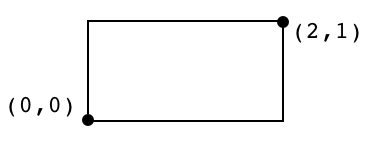
\includegraphics [scale=0.4] {dint1.png} \end{center}

We call the area element $dA = dx \ dy$ or $dy \ dx$, and write the integral as
\[ \iint f(x,y) \ dA =  \int \int f(x,y) \ dy \ dx \]

The double integral is the volume contained between the plane and the surface at $z$, within the bounds of the region $R$.  Write the bounds explicitly
\[ \iint_R f(x,y) \ dA =  \int_{x_1}^{x_2} \int_{y_1}^{y_2}  f(x,y) \ dy \ dx \]

\subsection*{iterated integral}

The idea is that if we slice the volume vertically perpendicular to the $x$ axis, we have a standard integral to yield the area of the slice when integrating over $dy$ parallel to the slice, and then in a second integral we add up all of these area slices over the range of $x$. 

\begin{center} 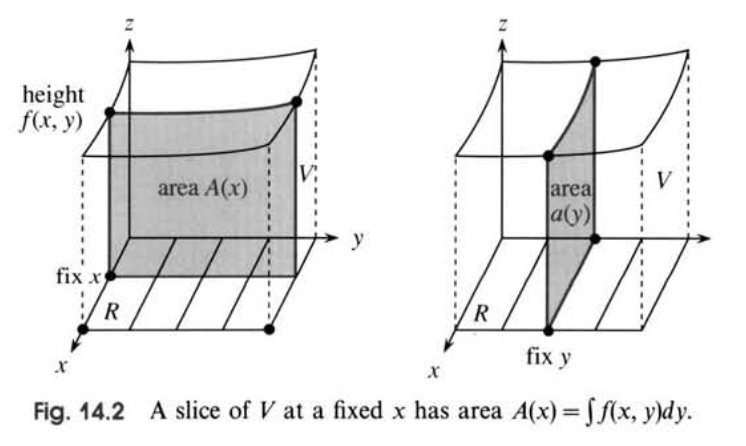
\includegraphics [scale=0.4] {iterated_integral.png} \end{center}

This is known as an \emph{iterated integral}.  The \emph{order of integration} refers to whether the slices are taken perpendicular to the $x$-axis ($\iint f(x,y) \ dy \ dx$) or perpendicular to the $y$-axis ($\iint f(x,y) \ dx \ dy$).

For this first example we sidestep one of the important complications of double integrals compared to single integrals.  Because the area is a rectangle, the bounds of $x$ and $y$ don't depend on where we are in the box, they are the same for each slice.

We have
\[ =  \int_{x = 0}^{2} \int_{y = 0}^{1}  f(x,y) \ dy \ dx \]
Suppose
\[ f(x,y) = xy^2 \]
For slices in the vertical direction (integrating over $dy$ first and $dx$ second), we have
\[ \int_{x=0}^{x=2} \int_{y=0}^{y=1} xy^2 \ dy \ dx \]

The notation says that we will do the integral with respect to $y$ first.  It is the \emph{inner} integral.
\[ \int_{y=0}^{y=1} xy^2 \ dy \]
As usual for multivariable calculus, in this computation we treat one variable, namely $x$, as a constant.  So we have
\[ \int_{y=0}^{y=1} xy^2 \ dy = \frac{1}{3} xy^3 \ \bigg |_{y=0}^{y=1} = \frac{1}{3}x \]
We plug this result into the outer integral
\[ \int_{x=0}^{x=2} \frac{1}{3}x  \ dx = \frac{1}{6} x^2 \ \bigg |_{x=0}^{x=2} = \frac{2}{3} \]

In general, you can switch the order of integration.  
\[ \int_{y_1}^{y_2}  \int_{x_1}^{x_2}  \ dx \ dy =\int_{x_1}^{x_2} \int_{y_1}^{y_2}  f(x,y) \ dy \ dx \]

There is a famous theorem due to Fubini that tells when this is allowed.  It will always be OK for us.

Sometimes we will only be able to compute a double integral one way (because we can't find the anti-derivative), but here we can do it the other way to check our result.
\[ \int_{y=0}^{y=1} \int_{x=0}^{x=2} xy^2 \ dx \ dy \]
Now, the inner integral is 
\[ \int_{x=0}^{x=2} xy^2 \ dx = \frac{1}{2} x^2y^2 \ \bigg |_0^2 = 2y^2 \]
and the outer integral is
\[ \int_{y=0}^{y=1} 2y^2 \ dy = \frac{2}{3}y^3 \ \bigg |_0^1 = \frac{2}{3} \]
The result is the same, so that looks good.

Let's do a second example.  Suppose we have the surface $f(x,y) = x^2 + y^2$,  a paraboloid surface opening up.  Our region R is the \emph{Cartesian product} 
\[ R = [-1,1] \times [0,1] \]

This notation means that $x$ lies on the interval $[-1,1]$ and $y$ on $[0,1]$.

We have 
\[ \int \int x^2 + y^2 \ dx \ dy \]
We can do this in either order, so we'll do the inner integral as
\[ \int_{-1}^1 x^2 + y^2 dx = \frac{1}{3}x^3 + xy^2 \ \bigg |_{-1}^{1} \]
\[ = \frac{1}{3} + y^2 - (-\frac{1}{3} - y^2) = \frac{2}{3} + 2y^2 \]
Now the outer integral is
\[ \int_0^1 \frac{2}{3} + 2y^2 \ dy = \frac{2}{3}y + \frac{2}{3}y^3  \ \bigg |_{0}^{1} \]
\[ = \frac{2}{3} + \frac{2}{3} = \frac{4}{3} \]

\subsection*{changed bounds}
More commonly, the shadow in the $xy$-plane is not a rectangle but instead, $x$ and $y$ are related by some function $y = f(x)$ or $x = f(y)$.

\begin{center} 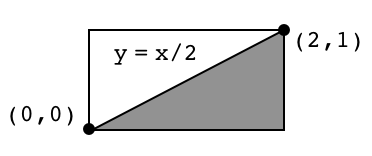
\includegraphics [scale=0.5] {dint2.png} \end{center}

Here, we use only half of the rectangle, the part that lies below the line $y=x/2$.  Now the upper bound, (the value of $y$) at the top of each slice changes depending on the value of $x$.

\begin{center} 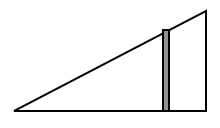
\includegraphics [scale=0.5] {dint3.png} \end{center}

When we integrate $dy$ first, the bounds are $y = [0, x/2]$
\[ \int_{x=0}^{x=2} \int_{y=0}^{y=x/2} xy^2 \ dy \ dx \]
The inner integral is
\[ \int_{y=0}^{y=x/2} xy^2 \ dy = \frac{1}{3} xy^3 \ \bigg |_{y=0}^{y=x/2} \]
\[ = \frac{1}{3}x(\frac{x}{2})^3 = \frac{1}{3} \ \frac{1}{8} \ x^4 \]
and the outer integral is 
\[ \int_{x=0}^{x=2} \frac{1}{3} \ \frac{1}{8}  x^4 \ dx = \frac{1}{3} \ \frac{1}{8}  \frac{x^5}{5} \ \bigg |_{x=0}^{x=2} \]
\[ = \frac{1}{3} \ \frac{1}{5} \ 4 = \frac{4}{15} \]

On the other hand, if we integrate $dx$ first, then the bounds for $x$ are $x=[2y, 2]$ and $y$ covers the entire range  $[0, 1]$. 
\begin{center} 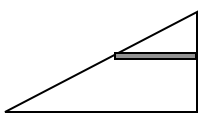
\includegraphics [scale=0.5] {dint4.png} \end{center}

 So we have
\[ \int_{y=0}^{y=1} \int_{x=2y}^{x=2} xy^2 \ dx \ dy \]
The inner integral is
\[ \int_{x=2y}^{x=2} xy^2 \ dy = \frac{1}{2}x^2y^2 \ \bigg |_{x=2y}^{x=2} = 2y^2 - 2y^4 \]
and the outer integral is
\[ \int_{y=0}^{y=1} 2y^2 - 2y^4 \ dy= \frac{2}{3}y^3 - \frac{2}{5}y^5 \ \bigg |_{y=0}^{y=1}  \]
\[ =  \frac{2}{3} - \frac{2}{5} =   \frac{10}{15} - \frac{6}{15} = \frac{4}{15}  \]

\subsection*{Strange limits}
Suppose we have a really simple function with a region whose boundary is something like $y = \ln x$.  We are interested in the region above the curve $y = \ln x$ and below $y=1$.  We go from $x=1$ (where $y=0$) to $x=e$ (where $y=1$).

\begin{center} 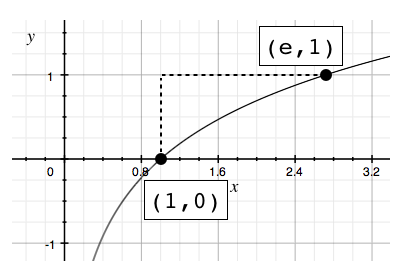
\includegraphics [scale=0.5] {dint5.png} \end{center}

Our simple function is just $1$.  When integrated over the region, this gives the area.
\[ \int \int_R 1 \ dA = A \]
If we integrate $dy$ first, our slices are vertical.  The bounds on $y$ are $[\ln x, 1]$.  The bounds for $x$ are $[1,e]$.
\[ \int_{x=1}^{x=e} \int_{y=\ln x}^{y=1} dy \ dx \]
The inner integral is
\[ y  \ \bigg |_{y=\ln x}^{y=1} = 1 - \ln x \]
and the outer integral is
\[ \int_{x=1}^{x=e} 1 - \ln x \ dx =  x - (x \ln x - x) \]
\[ = 2x - x \ \ln x \ \bigg |_{x=1}^{x=e} = 2e - e - 2 + 0 = e - 2 \]

If we do the integral with $dx$ first, we have
\[ \int_{y = 0}^{y=1} \int_{x=1}^{x=e^y} dx \ dy \]
The inner integral is
\[ \int_{x=1}^{x=e^y} dx = x \ \bigg |_{x=1}^{x=e^y} = e^y - 1  \]
and the outer integral is
\[ \int_{y=0}^{y=1}  e^y - 1  \ dy  = e^y - y \ \bigg |_0^1 \]
\[ = e - 1 - 1 + 0 = e - 2 \]

\subsection*{Only one way}
Next, consider
\[ \int \int_R e^{y^2} \ dA \]
We don't have a way to do $dy$ first
\[ \int  e^{y^2} \ dy = ? \]
However
\[ \int  e^{y^2} \ dx = e^{y^2} \ x \]
Now with just the right limits, we might have $x = [0,y]$, then
\[ \int_{x=0}^{x=y}  e^{y^2} \ dx = e^{y^2} \ x \ \bigg |_{x=0}^{x=y} = e^{y^2} \ y \]
We have the $y$ that we need and the outer integral is
\[ \int_{y=0}^{y=1}  e^{y^2} y \ dy = \frac{1}{2} e^{y^2} \ \bigg |_{y=0}^{y=1} = \frac{1}{2}(e-1) \]

\subsection*{Paraboloid example}
In his introduction to double integrals, Prof. Auroux describes the problem of finding the volume under the surface
\[ z = 1 - x^2 - y^2 \]
Visualizing surfaces can be difficult, but here, just set $x=0$ or $y=0$ (separately), then you see that we have a parabola.  This solid is a paraboloid, opening downward, with its apex at $(0,0,1)$.

\begin{center} 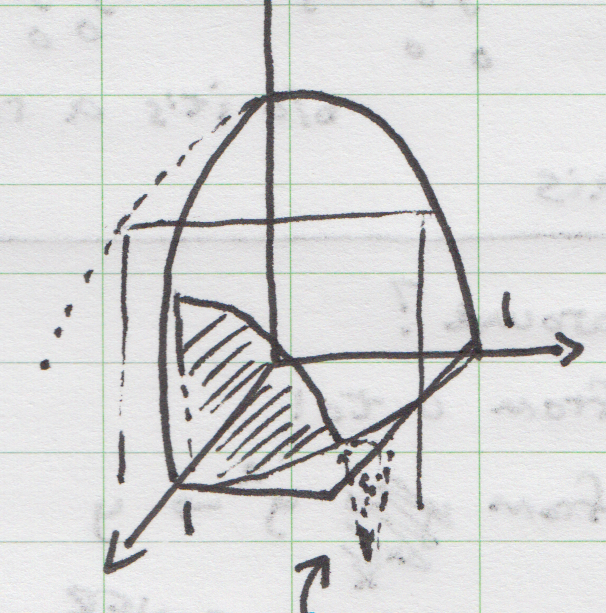
\includegraphics [scale=1.0] {dint.png} \end{center}

The first attempt integrates over the square region $[0,1] \times [0,1]$.  As he points out, this is a bit misguided, because for part of this region, the paraboloid is below the $x,y$-axis.  (If $x=y$ and $z=0$, $x = 1/\sqrt{2}$.  Nevertheless,

\[ \int_0^1 \int_0^1 1 - x^2 - y^2 \ dy \ dx \]
the inner integral is 
\[ y - x^2 y - \frac{1}{3}y^3  \ \bigg |_{0}^{1} = \frac{2}{3} - x^2 \]
and the outer one is
\[  \int_0^1 \frac{2}{3} - x^2 \ dx \]
\[ = \frac{2}{3} x - \frac{1}{3}x^3  \ \bigg |_{0}^{1} = \frac{1}{3} \]

The way to do this problem and actually obtain the volume of the quarter paraboloid is to set up the bounds of integration properly, over the quarter disk.  We can still have $x= [0,1]$ in the outer integral, but for the inner one we use $y=[0,\sqrt{1-x^2}]$.  The changed upper bound makes all the difference.  Now, we have

\[ \int_0^1 \int_0^{\sqrt{1-x^2}} 1 - x^2 - y^2 \ dy \ dx \]
the inner integral is 
\[ (1 - x^2) y - \frac{1}{3}y^3  \ \bigg |_{0}^{\sqrt{1-x^2}} \]
\[= (1-x^2) \sqrt{1-x^2} - \frac{1}{3} (1-x^2)^{3/2} \]
\[ = \frac{2}{3} (1-x^2)^{3/2} \]

Switch to polar coordinates for the outer integral (see the chapter \hyperref[sec:Change_of_variables]{\textbf{Change of variables}}):
\[ x = \sin \theta \]
\[ dx = \cos \theta \ d \theta \]
\[ \sqrt{1-x^2} = \cos \theta \]
we have
\[ = \frac{2}{3} \int \cos^3 \theta  \cos \theta \ d \theta \]
For the moment, just look it up
\[ = \frac{2}{3} \ [ \ \frac{\cos^3 \theta \ \sin \theta}{3} + \frac{3}{4}( \frac{\theta}{2} + \frac{1}{2} \sin \theta \ \cos \theta ) \ ]  \ \bigg |_{0}^{\pi/2}  \]

At the upper bound, $\cos \pi/2 = 0$ so we get
\[ \frac{2}{3} \ \frac{3}{4} \ \frac{1}{2} \ \frac{\pi}{2} \]
and at the lower bound, $\sin 0 = 0, \theta=0$ so we get $0$.  The result is $\pi/8$.

We will revisit the paraboloid later on.

\subsection*{Two curves}
In Auroux's second example, we have the line $y=x$ and the curve $x=y^2$.  These two curves cross at $(0,0)$ and $(1,1)$, with the line below the curve between these two endpoints.

\begin{center} 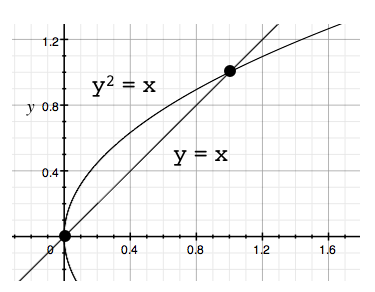
\includegraphics [scale=0.5] {dint6.png} \end{center}

If we integrate $dx$ first, the limits will be $x=y^2 \to x=y$, while if we integrate $dy$ first the limits are $y=x \to y=\sqrt{x}$.

Let's do the area function again ($f(x,y)=1$).
\[ \int \int_R 1 \ dA = ?\]
Start with $dx$ first
\[ \int_{y=0}^{y=1} \int_{x=y^2}^{x=y} \ dx \ dy\]
The inner integral is just
\[ \int_{x=y^2}^{x=y} \ dx  = x  \ \bigg |_{x=y^2}^{x=y} = y - y^2 \]
so the outer integral is
\[ \int_{y=0}^{y=1} y - y^2 \ dy = \frac{1}{2}y^2 - \frac{1}{3}y^3 \ \bigg |_{y=0}^{y=1} =  \frac{1}{2} - \frac{1}{3} = \frac{1}{6} \]
Doing it the other way
\[ \int_{x=0}^{x=1} \int_{y=x}^{y=\sqrt{x}} \ dy \ dx\]
The inner integral is
\[ \int_{y=x}^{y=\sqrt{x}} \ dy  = y  \ \bigg |_{y=x}^{y=\sqrt{x}} = \sqrt{x} - x \]
so the outer integral is
\[ \int_{x=0}^{x=1}\sqrt{x} - x \ dx = \frac{2}{3} x^{3/2} - \frac{1}{2}x^2  \ \bigg |_{x=0}^{x=1} = \frac{2}{3} - \frac{1}{2} = \frac{1}{6} \]


\end{document}